\chapter{Trajectory patterns}\label{trajectories}
\section{Introduction}
This GSP attempts to identify people’s movement patterns from anonymized wifi logs. \autoref{hernoemen} described movement patterns including spatial and temporal aspects of single movements of a crowd of people. Another way of looking at movements, is by tracking individual movement for a longer time interval. A large set of individual trajectories can be used for the identification of typical movements among users of the campus. The method uses concepts from sequential pattern mining. \\\\
This chapter presents a method for identifying movement patterns using individual trajectories. As described in \autoref{movementpatterns}, if moving individuals share some locations in their trajectory, you can speak of co-location in space. When the order of the shared locations are similar for multiple trajectories, you can speak of typical movement. This concept is explored for the identification of movement patterns, and thus the usage of the campus. This approach can answer different questions than looking at single movements, as is done in \autoref{hernoemen}. For example, ‘how many places the user frequently visits’, ‘at what order the user visits places’, ‘how often a trajectory happens’, ‘how many places contained in a frequent trajectory’.\\\\
First, this chapter will describe the problem description, including the extraction of locations of a user, the mining of individual trajectories from an anonymized Wi-Fi scan list, and finaly the mining of movement patterns from a set of trajectories using the PrefixSpan algorithm.
\section{Problem description}
% schrijf ff intro hier
\subsection{Location extraction}
The data provided by the eduroam network enables a detailed view of people’s movement on campus. The large coverage of the eduroam network allows to track users for a large part of the day when they enter the campus. However, the observation space is limited to the extent of the size of the campus, making it not possible to track people outside the eduroam network. A second disadvantage is the spatial resolution of the positioning method. The range a mobile device can be connected to an AP,  influences the accuracy of the estimated location of a mobile device. For indoor environments of the TU Delft campus, this is just a few tens of meters wide. This resolution allows tracking movement at a building level by re-locating mobile devices to the closest AP. Data between two re-locations is not available. Therefore, an individual’s trajectory is depicted by connecting the re-locations as a sequence of APs. These individual trajectories are used to identify patterns. \\\\
A location represents a geographic position where a user stays, i.e. a user is in state. For identifying movement patterns from Wi-Fi monitoring, we are interested in movement between two locations where an individual stays for a longer time period. Such a location, or stay place, can be detected when a user is connected to the same AP for a longer time. To detect  buildings as a location (i.e. contains multiple APs), two consecutive Wi-Fi scans must contain  APs of the same building. With a data collecting interval of 5 minutes, it means that people will be filtered out if their stay duration is less than 10 minutes. Based on this assumption, people with a shorter stay duration are considered passing by, as explained in \autoref{preprocessing}.

\subsection{Individual trajectory}
An individual’s trajectory is constructed as a sequence of locations in order of the scan time. Start and end time of a trajectory can be specified with a time interval. Two consecutive scans from the Wi-Fi log are considered in the same trajectory if and only if \textit{$t_{s2}$ - $t_{e1}$} \textless \textit{$T_{split}$}, where \textit{$T_{split}$} is the splitting threshold. The splitting threshold is important when dealing with people, who are not observed for a long duration of time, i.e. people moving home. For example, if a student leaves the campus at the end of the day, and returns the next morning, seperate trajectories should be created. Because, \textit{$T_{split}$} is larger than the threshold for identifying \textit{'world'} (see \autoref{preprocessing}), the trajectory will always start and end with \textit{'world'}. If \textit{p} is a location, then a trajectory can be written as:
$$p_{1} \rightarrow p_{2} \rightarrow p_{3} \rightarrow …\rightarrow p_{n}$$
Given a time interval, there is a set of individual trajectories $\textit{S} = \{t_{1}, t_{2}, t_{3},...,t_{n}\}$ where each $t_{i}$ is the trajectory. 

\subsection{Trajectory Pattern}
From a set \textit{S} of trajectories, different patterns can be identified using sequential pattern mining algorithms. Frequency of a trajectory by all users of the campus can be detected. This can be represented as a trajectory \textit{T} with a support \textit{s}. Support means how many times the same sequence, or sub-sequence, is shared in the set of trajectories. This gives valuable information on the order common buildings are used and what order of buildings occurs the most. Using a minimum support threshold, sequential mining returns all movement patterns that satisfy \textit{n} \textgreater 2 and support \textit{T} \textgreater \textit{$S_{min}$}   Furthermore, the length of common trajectories can be discovered. This allows for identification of movement patterns of a specific length \textit{n}. Also, when location is not considered, but only the length of a trajectory, the mobility pattern of an individual can be described in terms of how many times he/she re-locates. \autoref{figure:figseqpattern} illustrates a trajectory pattern of lenght 3, and has a support of 3.

\begin{figure}[H]
\centering
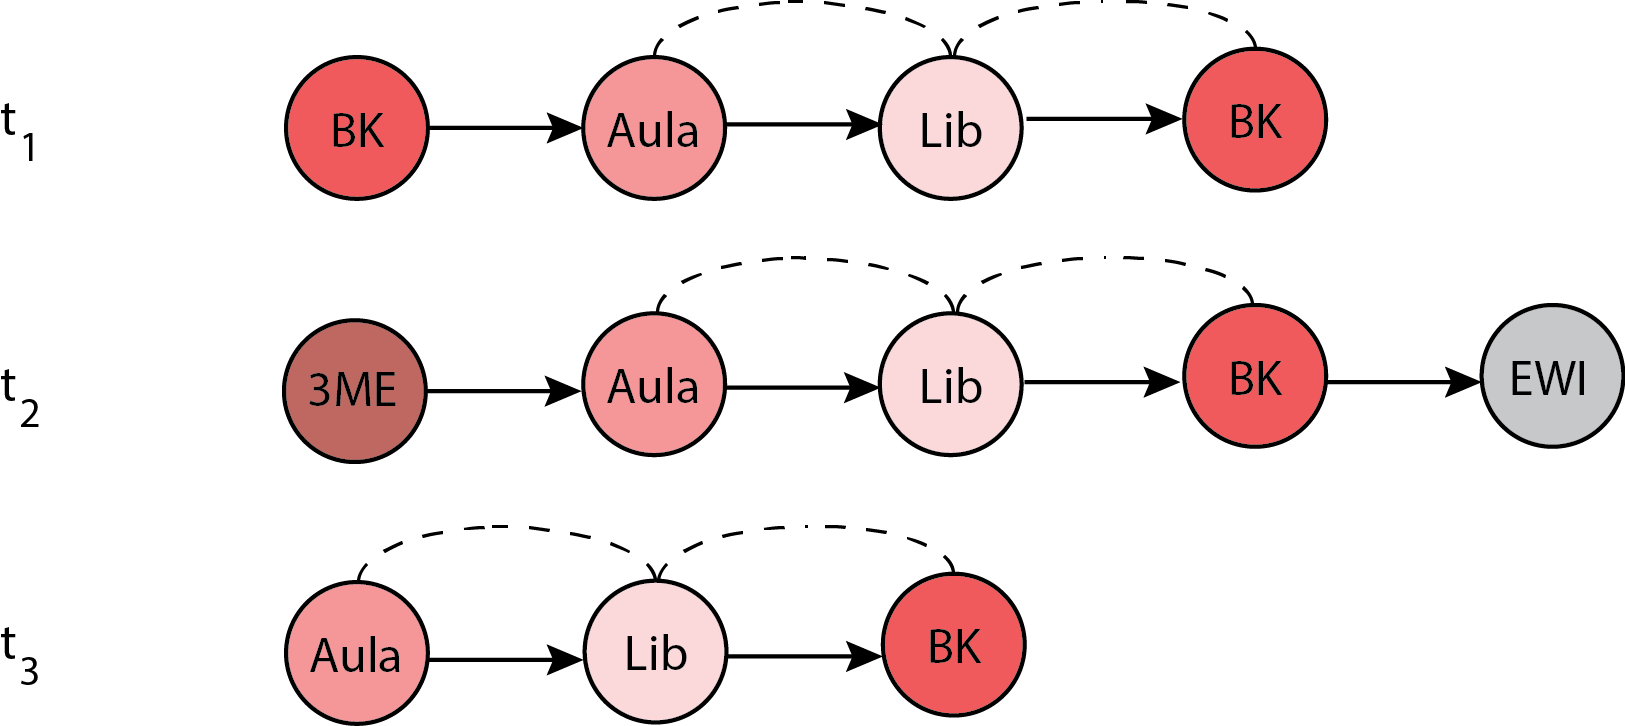
\includegraphics[scale=0.8]{sub-sequence-pattern.png}
\captionsetup{justification=centering}
\caption{sample of individual trajectories}
\label{figure:figseqpattern}
\end{figure}

For this study, a trajectory pattern is a sequence of states with \textit{n} \textgreater 2 and support \textgreater \textit{$S_{min}$}. We are only considering trajectory patterns with \textit{n} \textgreater 2, because \autoref{hernoemen} already looked at two consecutive states.\\\\
There exists many developed sequential pattern mining algorithms. For this study PrefixSpan \cite{pei2004mining} is used to identify common shared trajectories or sub-trajectories. This sequential pattern mining algorithm can find re-occuring sequences or sub-sequences from a set of trajectories. For every common sequence, a support value is computed. 
\section{Implementation}
For this analyses the same data is used as for the single movement analysis. As described in \autoref{preprocessing}, from the raw Wi-Fi log states are extracted. More than 2.8 million states are identified from the dataset. This information is stored including a unique mac address, a number representing a building, the start time of the state and the end time of the state. The states are used to construct individual sequences ordered by date and time. The \textit{$T_{split}$} is used to create separate trajectories for different days, for each individual. For this study, a new trajectory is created when there has not been a connection for 5.5 hours, i.e. a state of outside campus ('world') > 5.5 hours. This threshold is suitable for identifying people moving home at the end of the day and coming back the next morning. After splitting the sequences, over 950.000 trajectories are created, with temporal granularity of one day. Every trajectory starts and ends with 'world', i.e. people start and end there trajectory outside the campus. A sample of a constructed trajectory can be seen in \autoref{figure:figtrajectory}

\begin{figure}[H]
\centering
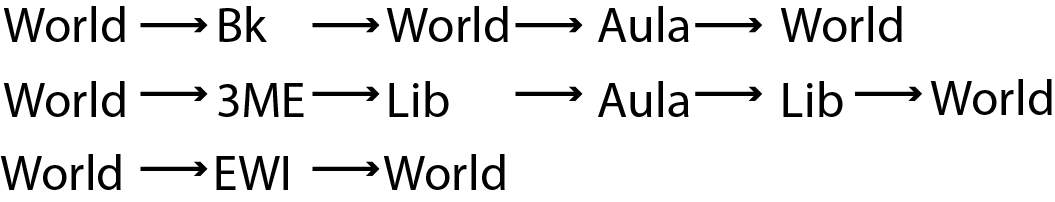
\includegraphics[scale=0.5]{sampleTraject.png}
\captionsetup{justification=centering}
\caption{sample of individual trajectories}
\label{figure:figtrajectory}
\end{figure}

Based on the created trajectories, trajectory patterns with a suppport value are detected by applying the PrefixSpan algorithm. \autoref{figure:prefixspan} shows an example of the detection of patterns with a support value given by the sequential pattern algorithm. Logically, the pattern with the highest support is a lenght-1 sequence. The longer patterns get, the lower the support will be.  

\begin{figure}[H]
\centering
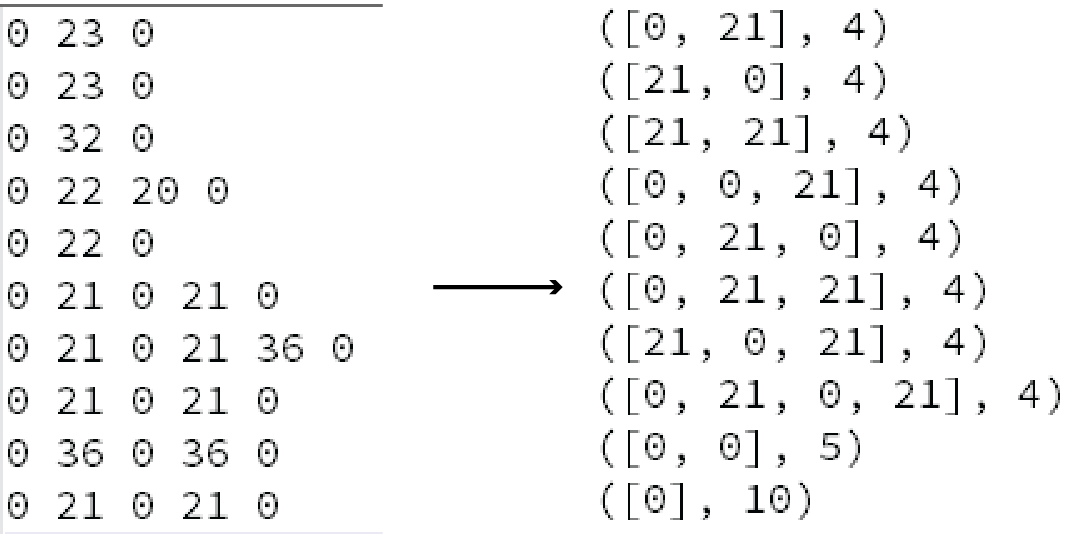
\includegraphics[scale=0.8]{prefixspan.png}
\captionsetup{justification=centering}
\caption{sample of individual trajectories}
\label{figure:prefixspan}
\end{figure}


 
\section{Results}
% <-- Please divide into the correct sections! --> %





